\documentclass[xelatex,ja=standard,jafont=noto]{bxjsarticle}
\usepackage[utf8]{inputenc}

\date{11.4 2020}

\usepackage{natbib}
\usepackage{graphicx}
\usepackage{tikz}
\usepackage{circuitikz}
\usepackage{tabularx}
\usepackage{diagbox}
\usepackage{amsmath,amssymb}
\numberwithin{figure}{section}
\usepackage{pdfpages}

\usepackage{hyperref}


\begin{document}
\renewcommand{\figurename}{Fig.}
\renewcommand{\tablename}{Table }



	\begin{titlepage}
			\begin{center}
				
				{\Large 令和2年}
				
				\vspace{10truept}
				
				{\Large 機械工学実験2}
				
				\vspace*{140truept}
				
				{\Huge モータシステムの制御系設計} 
				
				\vspace{160truept}
				
				{\Large 指導教員}
				
				\vspace{10truept}
				
				{\Large  Ito Kazuhisa }
				
				\vspace{70truept}
				{\Large 芝浦工業大学}
				
				\vspace{10truept}
				
				{\Large 機械制御システム}
				
				\vspace{30truept}
				
				{\Large bq18026 関宇}      
				
			\end{center}
		\end{titlepage}
%\includepdf[pages={1}]{sd.pdf}


\tableofcontents

\newpage



\section{実験の目的}

機械システムを解析あるいは制御する際に用いられる数学モデルに基づく考え方は既に多くの専門科
目で学んだものであるが,多くの利点を持つ.本テーマでは,最も身近な例であるモータの回転角度制
御系を取り上げ,モデルベースアプローチの概要および簡単な設計手順を学ぶことを目的とする.


PID制御の構成、役割を理解すること.

PIDパラメータの影響、設定基準

モータの制御系設計とその評価


\section{実験道具}

MATLAB2019R, MinSeg.com[TSI-Minseg-001Kit]

\section{実験手順}

\subsection{モータのパラメータ同定(同定実験)}
摩擦などの一般的にはゲイン K および時定数 T などのパラメータは理論的に求められないことが多い.これらを実験により求めることをパラメータ同定,またはシステム同定という.\\

\begin{figure}[h!]
    \centering
    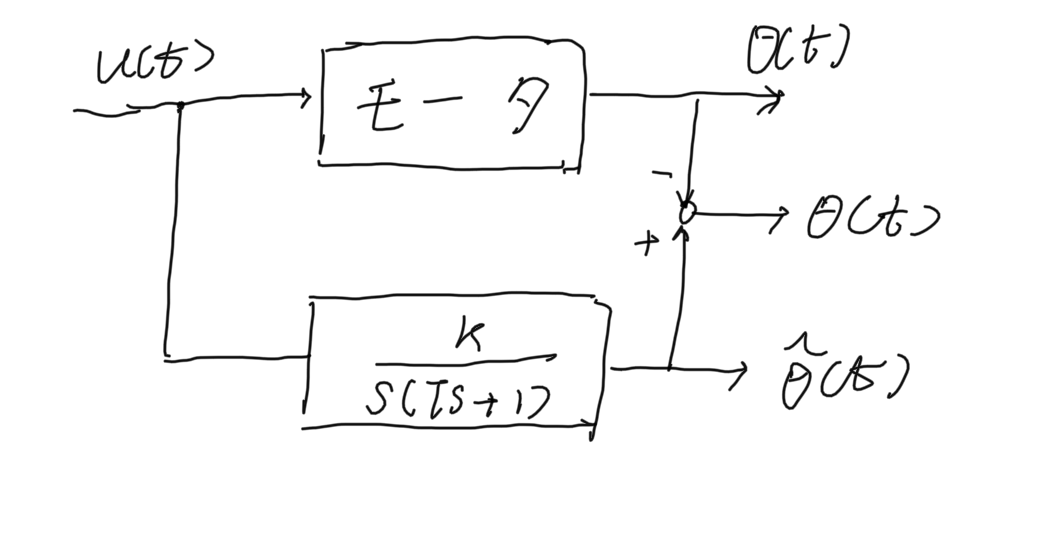
\includegraphics[scale=0.3]{019.png}
    \caption{fs=(4/3)fn}
\end{figure}

モータ系に色んな入力に対する出力を測って、それをコンピュータ上で計算した伝達関数の出力の数値と比較して、TとKの値が大体推測することができる.具体的に、推定値と実際値の差が0くらいになるようなKとTはこのシステムのTとKと当てていると言える.\\


しかしモータシステムに対して積分作用を持っているから、もしステップ入力を選ぶと出力が発散することが起きるので、定数フィードバックによる閉ループ系を構成することで安定化を行ったシステムに対して実験を行う. 

\newpage

そこでパラメータ同定用システムの伝達関数は

\begin{equation}
    G(s)=\frac{\frac{KK_{P}}{s(Ts+1)}}{1+\frac{KK_{P}}{s(Ts+1)}}=\frac{KK_{P}}{s^{2}T+s+KK_{P}}
\end{equation}\\

こうやってフィードバック系を組んで出力の最終値を1になることができる.実験の結果を最大誤差および式 (2) で定義される二乗平均平方根誤差 $e_{RMS}$ にて評価し,ゲイン K と時定数 T を推定する.

\begin{equation}
    e_{RMS}=\sqrt{\frac{1}{n}\sum_{i=1}^{n}e^{2}(i)},e(i)=\theta(i)-\hat{\theta}(i)
\end{equation}

ただし,n はデータ点数,$θ$は計測されたモータ回転角度,$\hat{\theta}$は数学モデルにより計算されたモータ回転角度である.同定実験のデータを表のようにまとめる.

\begin{table}[!htbp]
\centering
\caption{<同定実験データ>}
\begin{tabular}{cccccc}
\hline
 $ K_{P}$ & $T_{fit}$ & $e_{RMS}$ & $e_{max}$& $K$ & $T$\\
\hline
2& 1& 0.051& 0.147&8.068& 0.237\\
 2& 1.25& 0.049&0.130&7.490&0.224\\
2 & 1.5&0.049 &0.132&7.428&0.221\\
\hline
\end{tabular}
\end{table}

実験データによって、$K_{P}=2,T_{fit}=1.25$を選定した時の最大誤差、二乗平均平方根誤差が共に小さいので、この条件で実際のK,Tを選定する.つまり、




\begin{equation}
    K=7.490,T=0.224;
\end{equation}

\subsection{モータの制御系設計}


求められたパラメータに対して比例微分先行型積分制御およびフィードフォワード制御を組合せた系
(I-PD+FF 制御) を設計する. 指定したオーバシュート
量と整定時間を満たすような PDゲインおよびフィードフォワードゲイン $K_{FF}$ を設計する.\\

目標値信号r の変化の影響を直接に受けないよう,
比例制御および微分制御系部をモータ出力のフィードバックとしたI-PD制御系を構成する.このシステムの伝達関数は$K_{FF}=0$の時の伝達関数と一致するので、

\begin{equation}
    G(s)=\frac{\frac{K_{I}}{s}\cdot\frac{K}{Ts^{2}+(KK_{D}+1)s+KK_{P}}}{1+\frac{K_{I}}{s}\cdot\frac{K}{Ts^{2}+(KK_{D}+1)s+KK_{P}}}
\end{equation}

\begin{equation}
    =\frac{KK_{I}}{s^{3}+s^{2}(KK_{D}+1)+sKK_{P}+KK_{I}}
\end{equation}

これを設計にして、ある伝達関数に一致させるようなことができれば、もしその伝達関数を指定すれば、逆に$K_{P},K_{I},K_{D}$が決まることになる.\\


    実験で制御したいのは、5パーセントの整定時間、最大オーバーシュート量と$\alpha$である.もし整定時間、最大オーバーシュート量は二次遅れ系のパラメータの$\zeta,\omega_{n}$とは何か関連性があればうまくPIDパラメータが決まることができる.
    
\section{制御実験データおよび評価}

\subsection{実験データ}

選ぶ $\alpha$については,虚軸に近いものとそうでないものの二通りを選ぶことで、今回の実験で20,1,20,1,200の順で実験を行うことにする.

\begin{table}[!htbp]
\centering
\caption{<制御実験データ>}
\begin{tabular}{ccccccccc}
\hline
 $ K$ & $T$ & $M_{P}$ & $T_{s}$& $\alpha$ & $K_{p}$&$K_{i}$&$K_{d}$&$K_{ff}$\\
\hline
7.49& 0.22 & 0.5& 1 & 20 & 9.38 & 115.83 & 0.64 &0\\
\hline
 7.49&  0.22&  0.5& 1 &1 &5.97 &5.79 & 0.08&0 \\
 \hline
7.49 &  0.22& 0.5 &1 &20 & 9.38 & 115.83& 0.64&5.79\\
\hline
7.49 &  0.22& 0.5 &1 &1 & 5.97 & 5.79& 0.08 &5.79\\
\hline
7.49 &  0.22& 0.5 &1 &200 & 41.64&1158.27 & 6.02 &0\\
\hline
\end{tabular}
\end{table}


得られた実験データをグラフにまとめる.

\begin{figure}[h!]
    \centering
    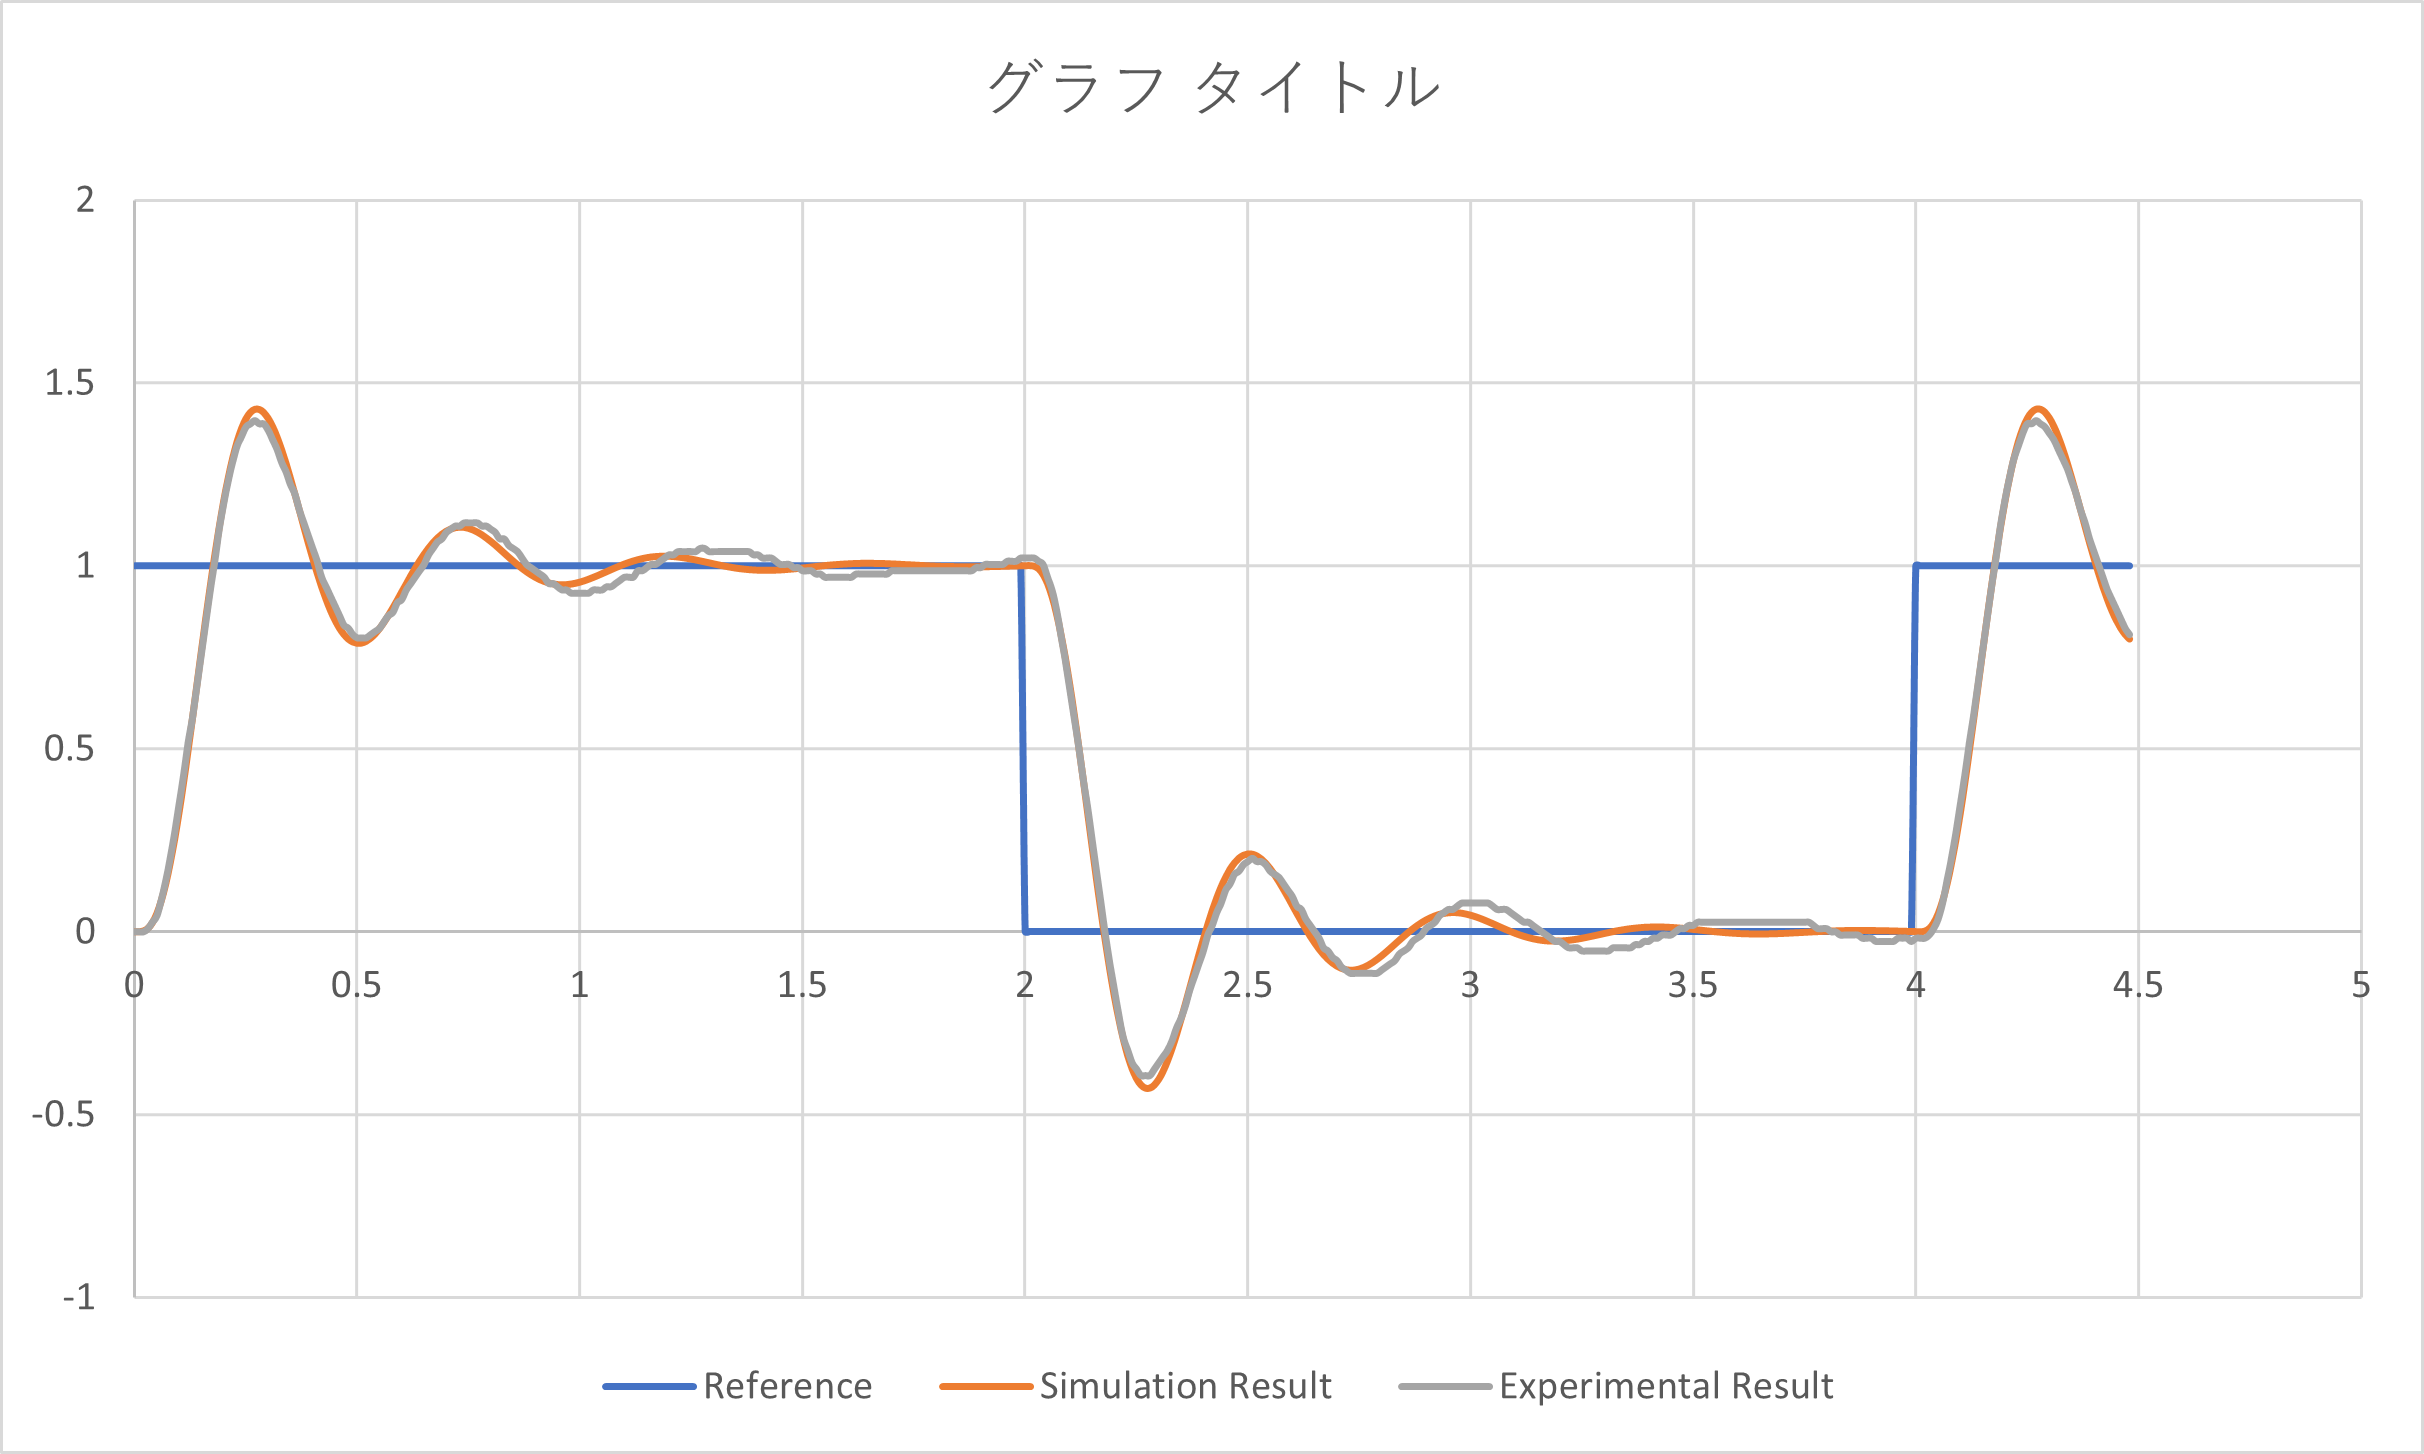
\includegraphics[scale=0.6]{020.png}
    \caption{$\alpha=20,K_{ff}=0$}
\end{figure}

\newpage

\begin{figure}[h!]
    \centering
    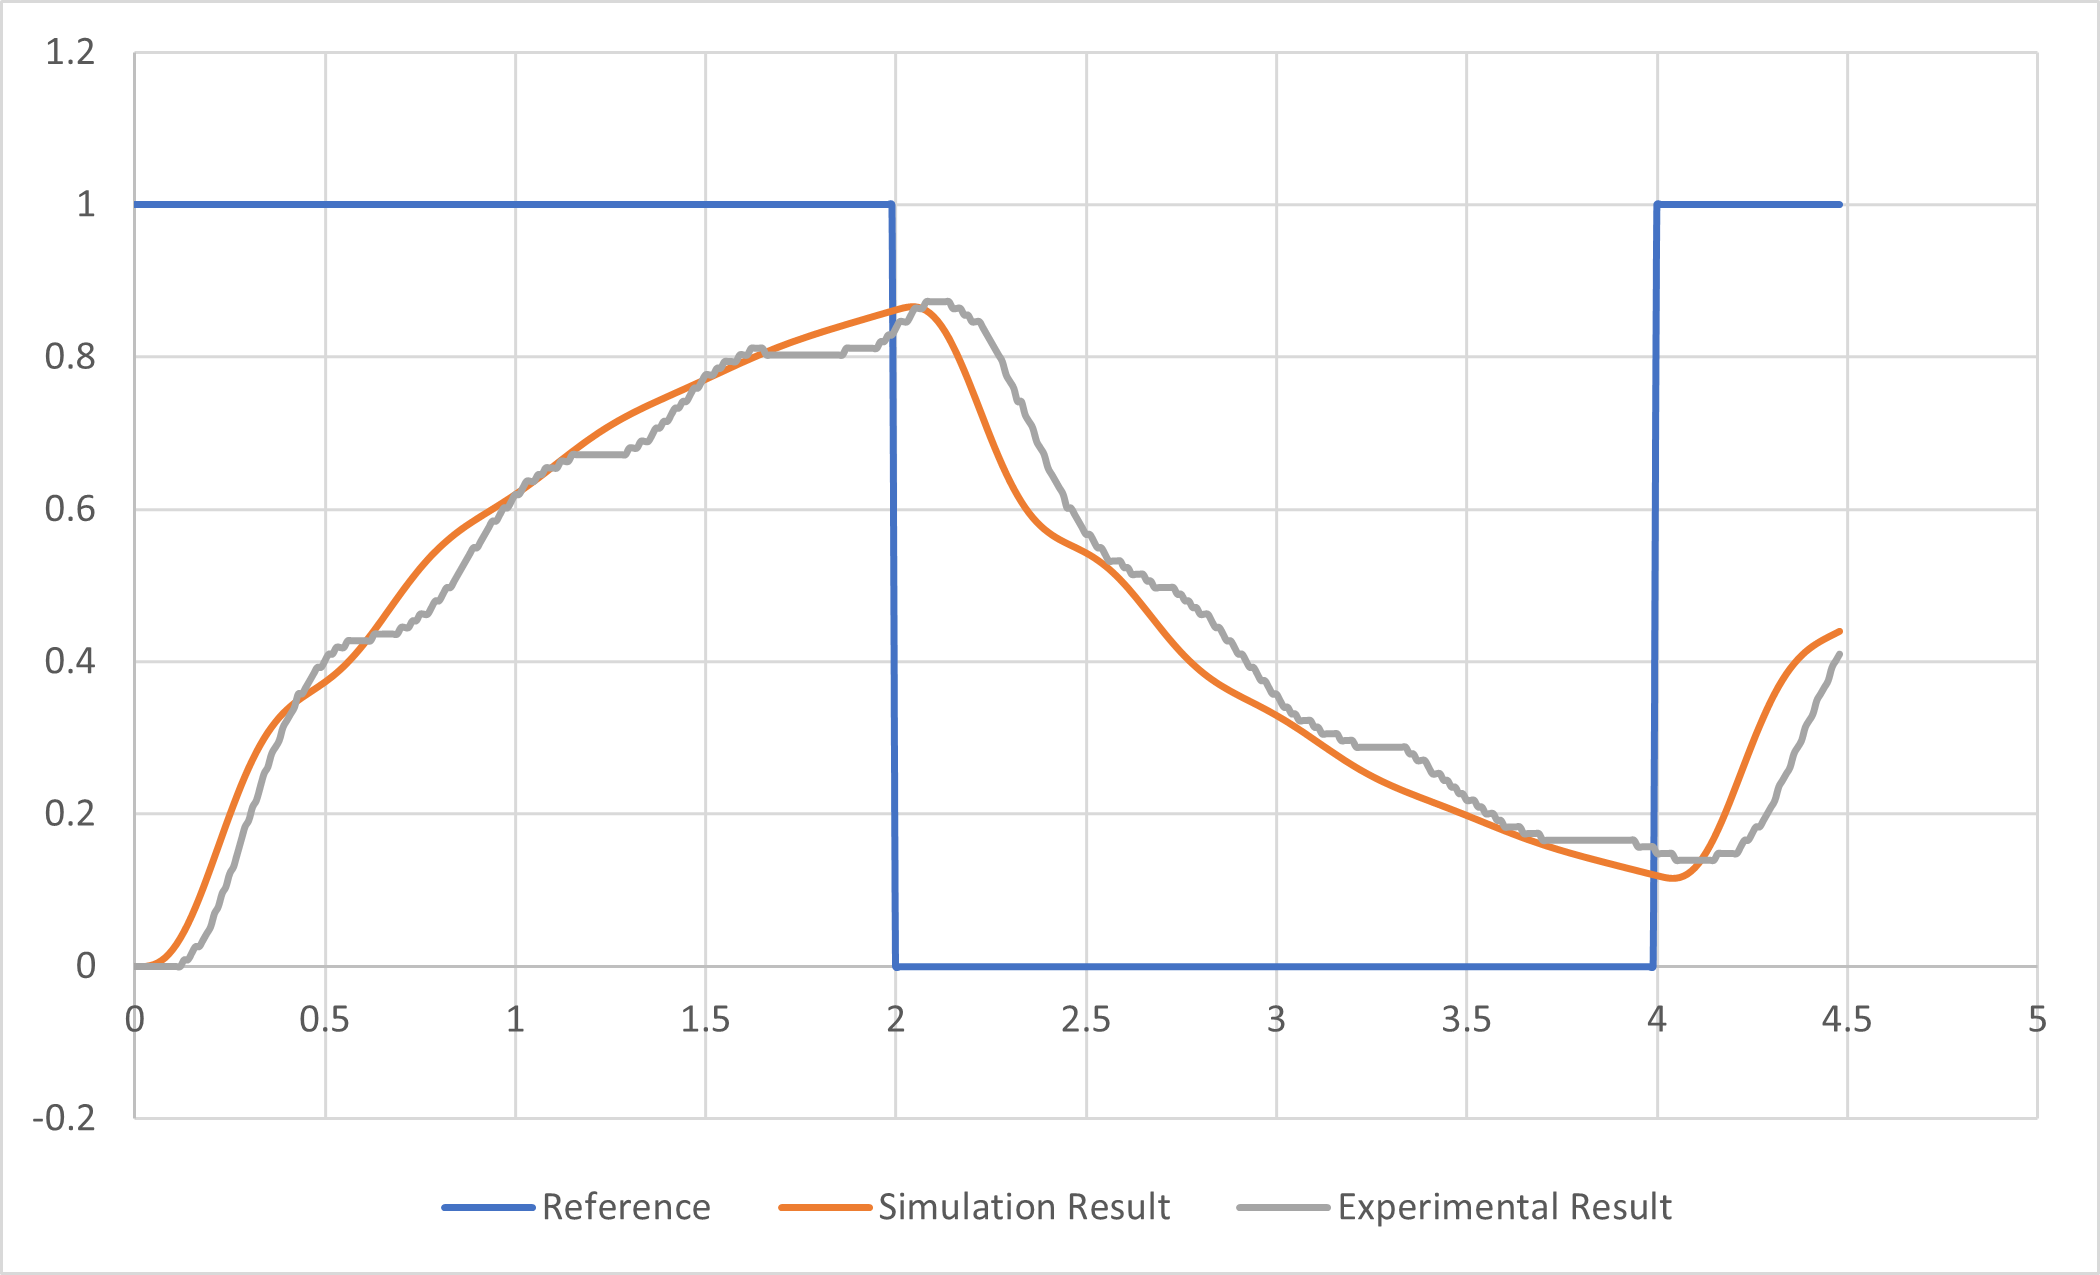
\includegraphics[scale=0.7]{021.png}
    \caption{$\alpha=20,K_{ff}=0$}
\end{figure}

\begin{figure}[h!]
    \centering
    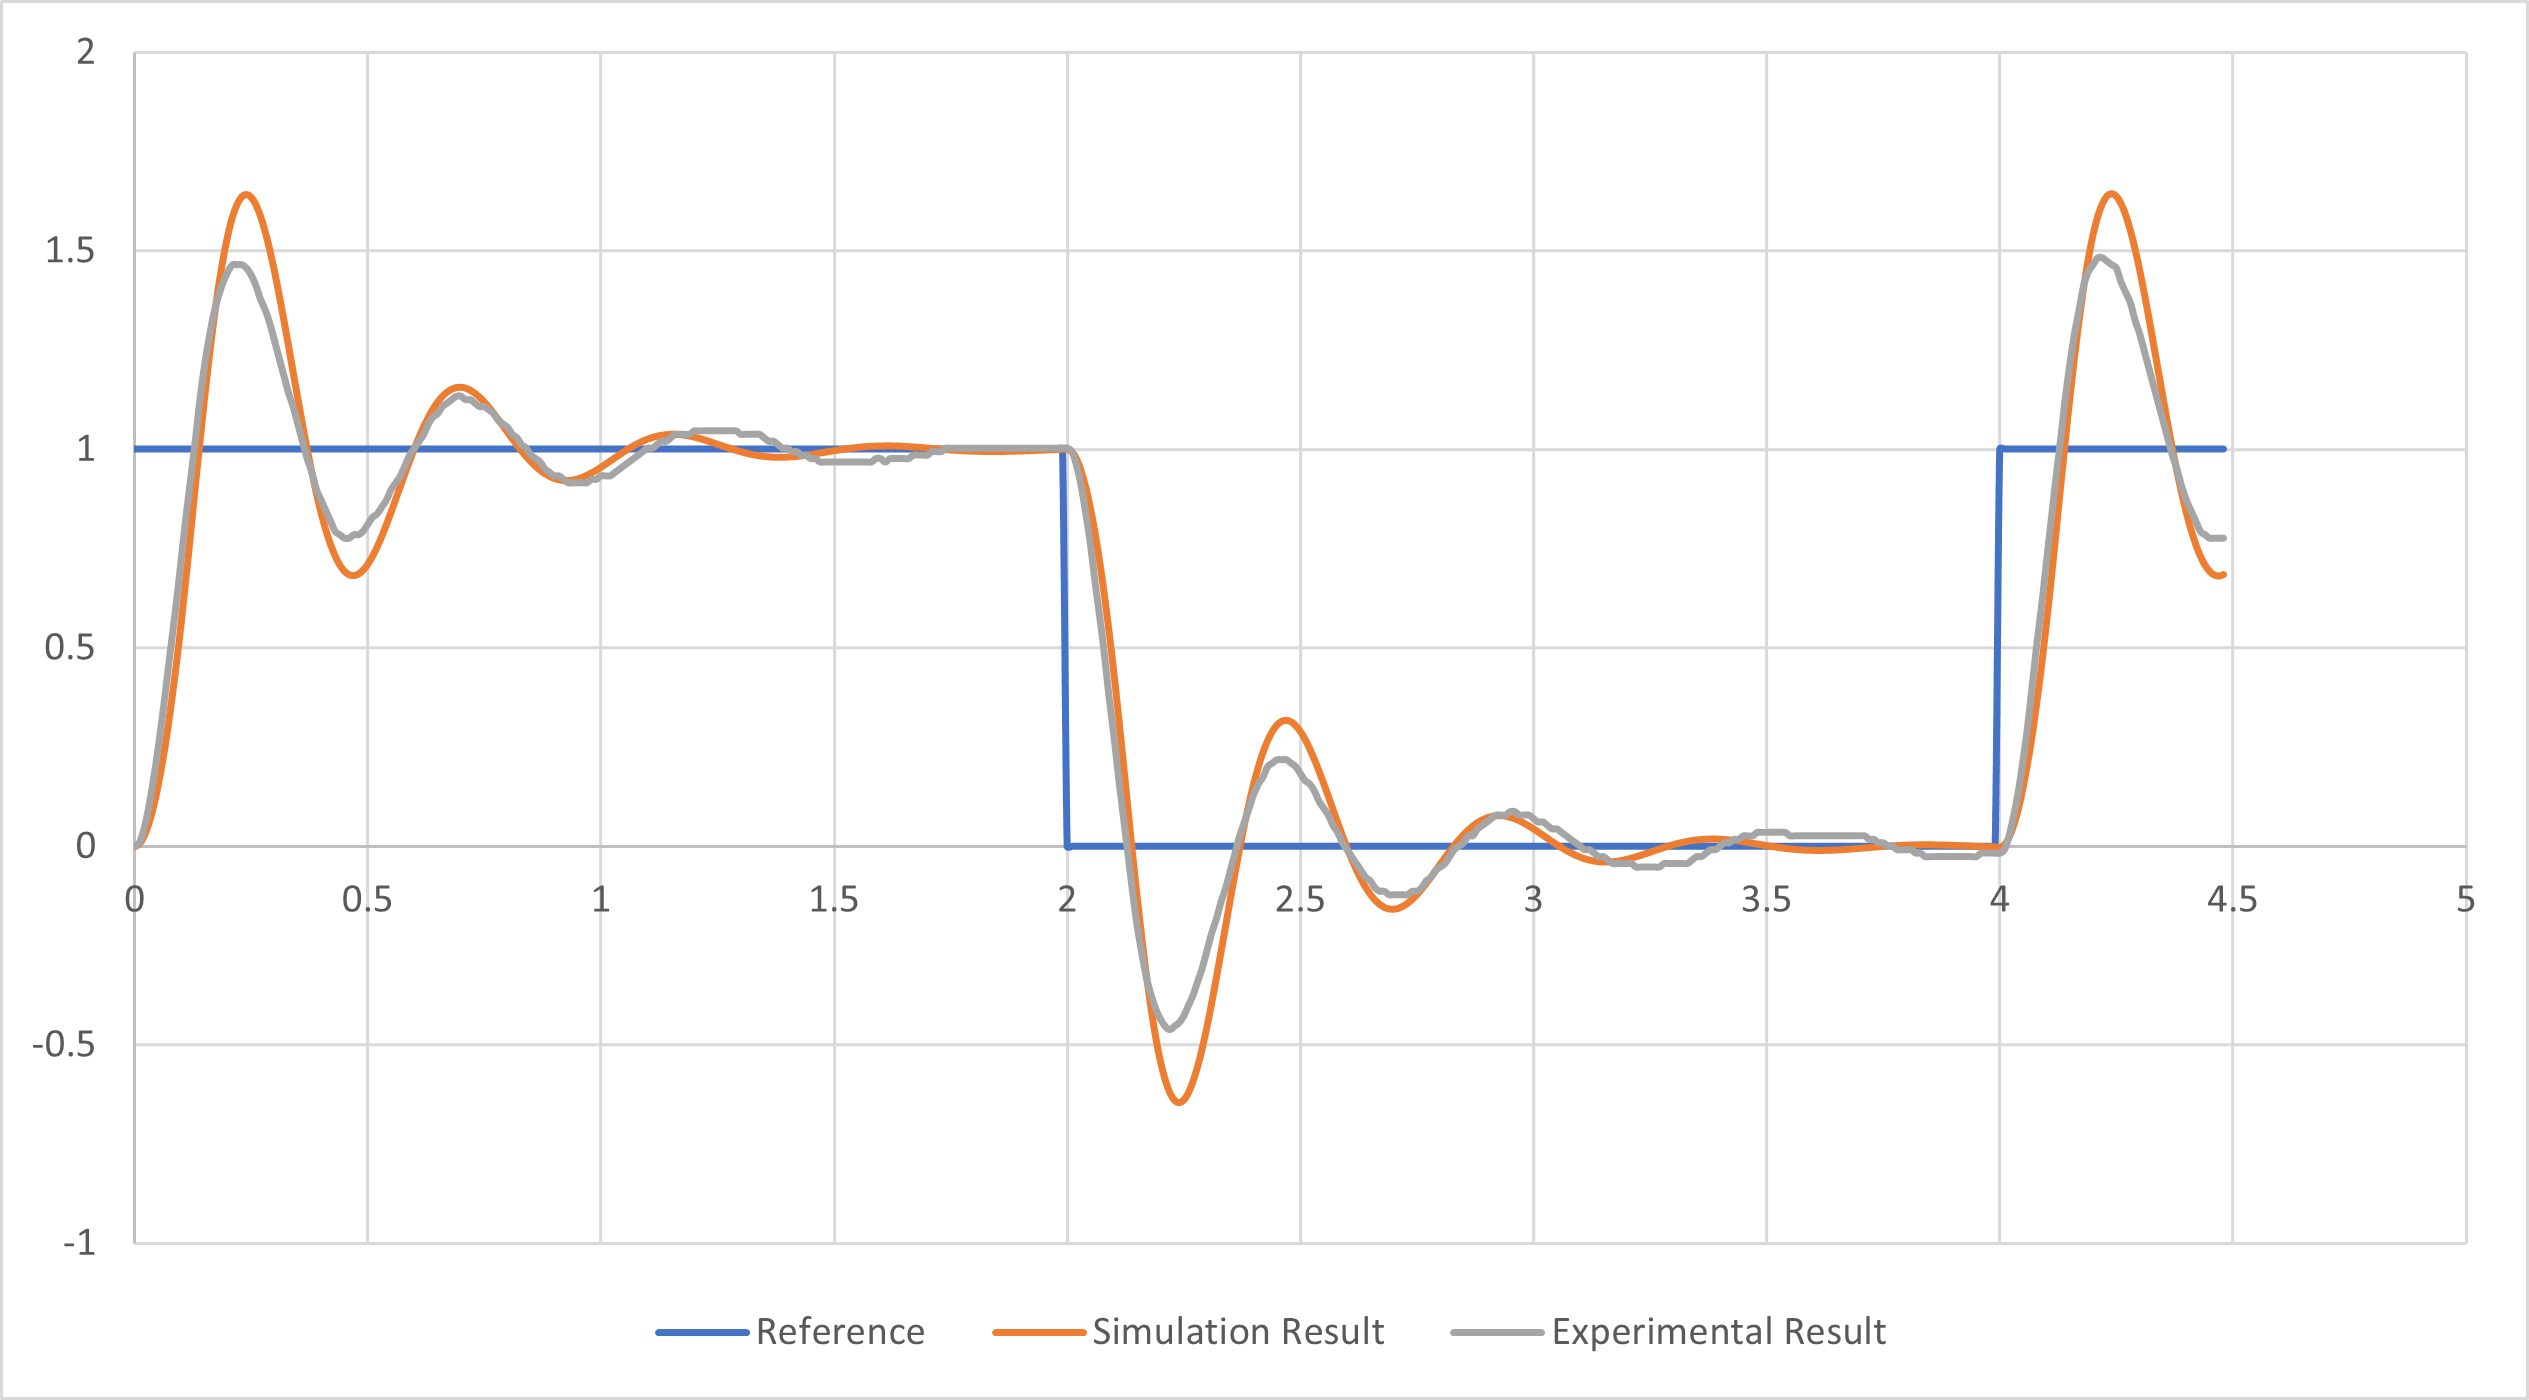
\includegraphics[scale=0.6]{022.png}
    \caption{$\alpha=20,K_{ff}=5.79$}
\end{figure}


\newpage

\begin{figure}[h!]
    \centering
    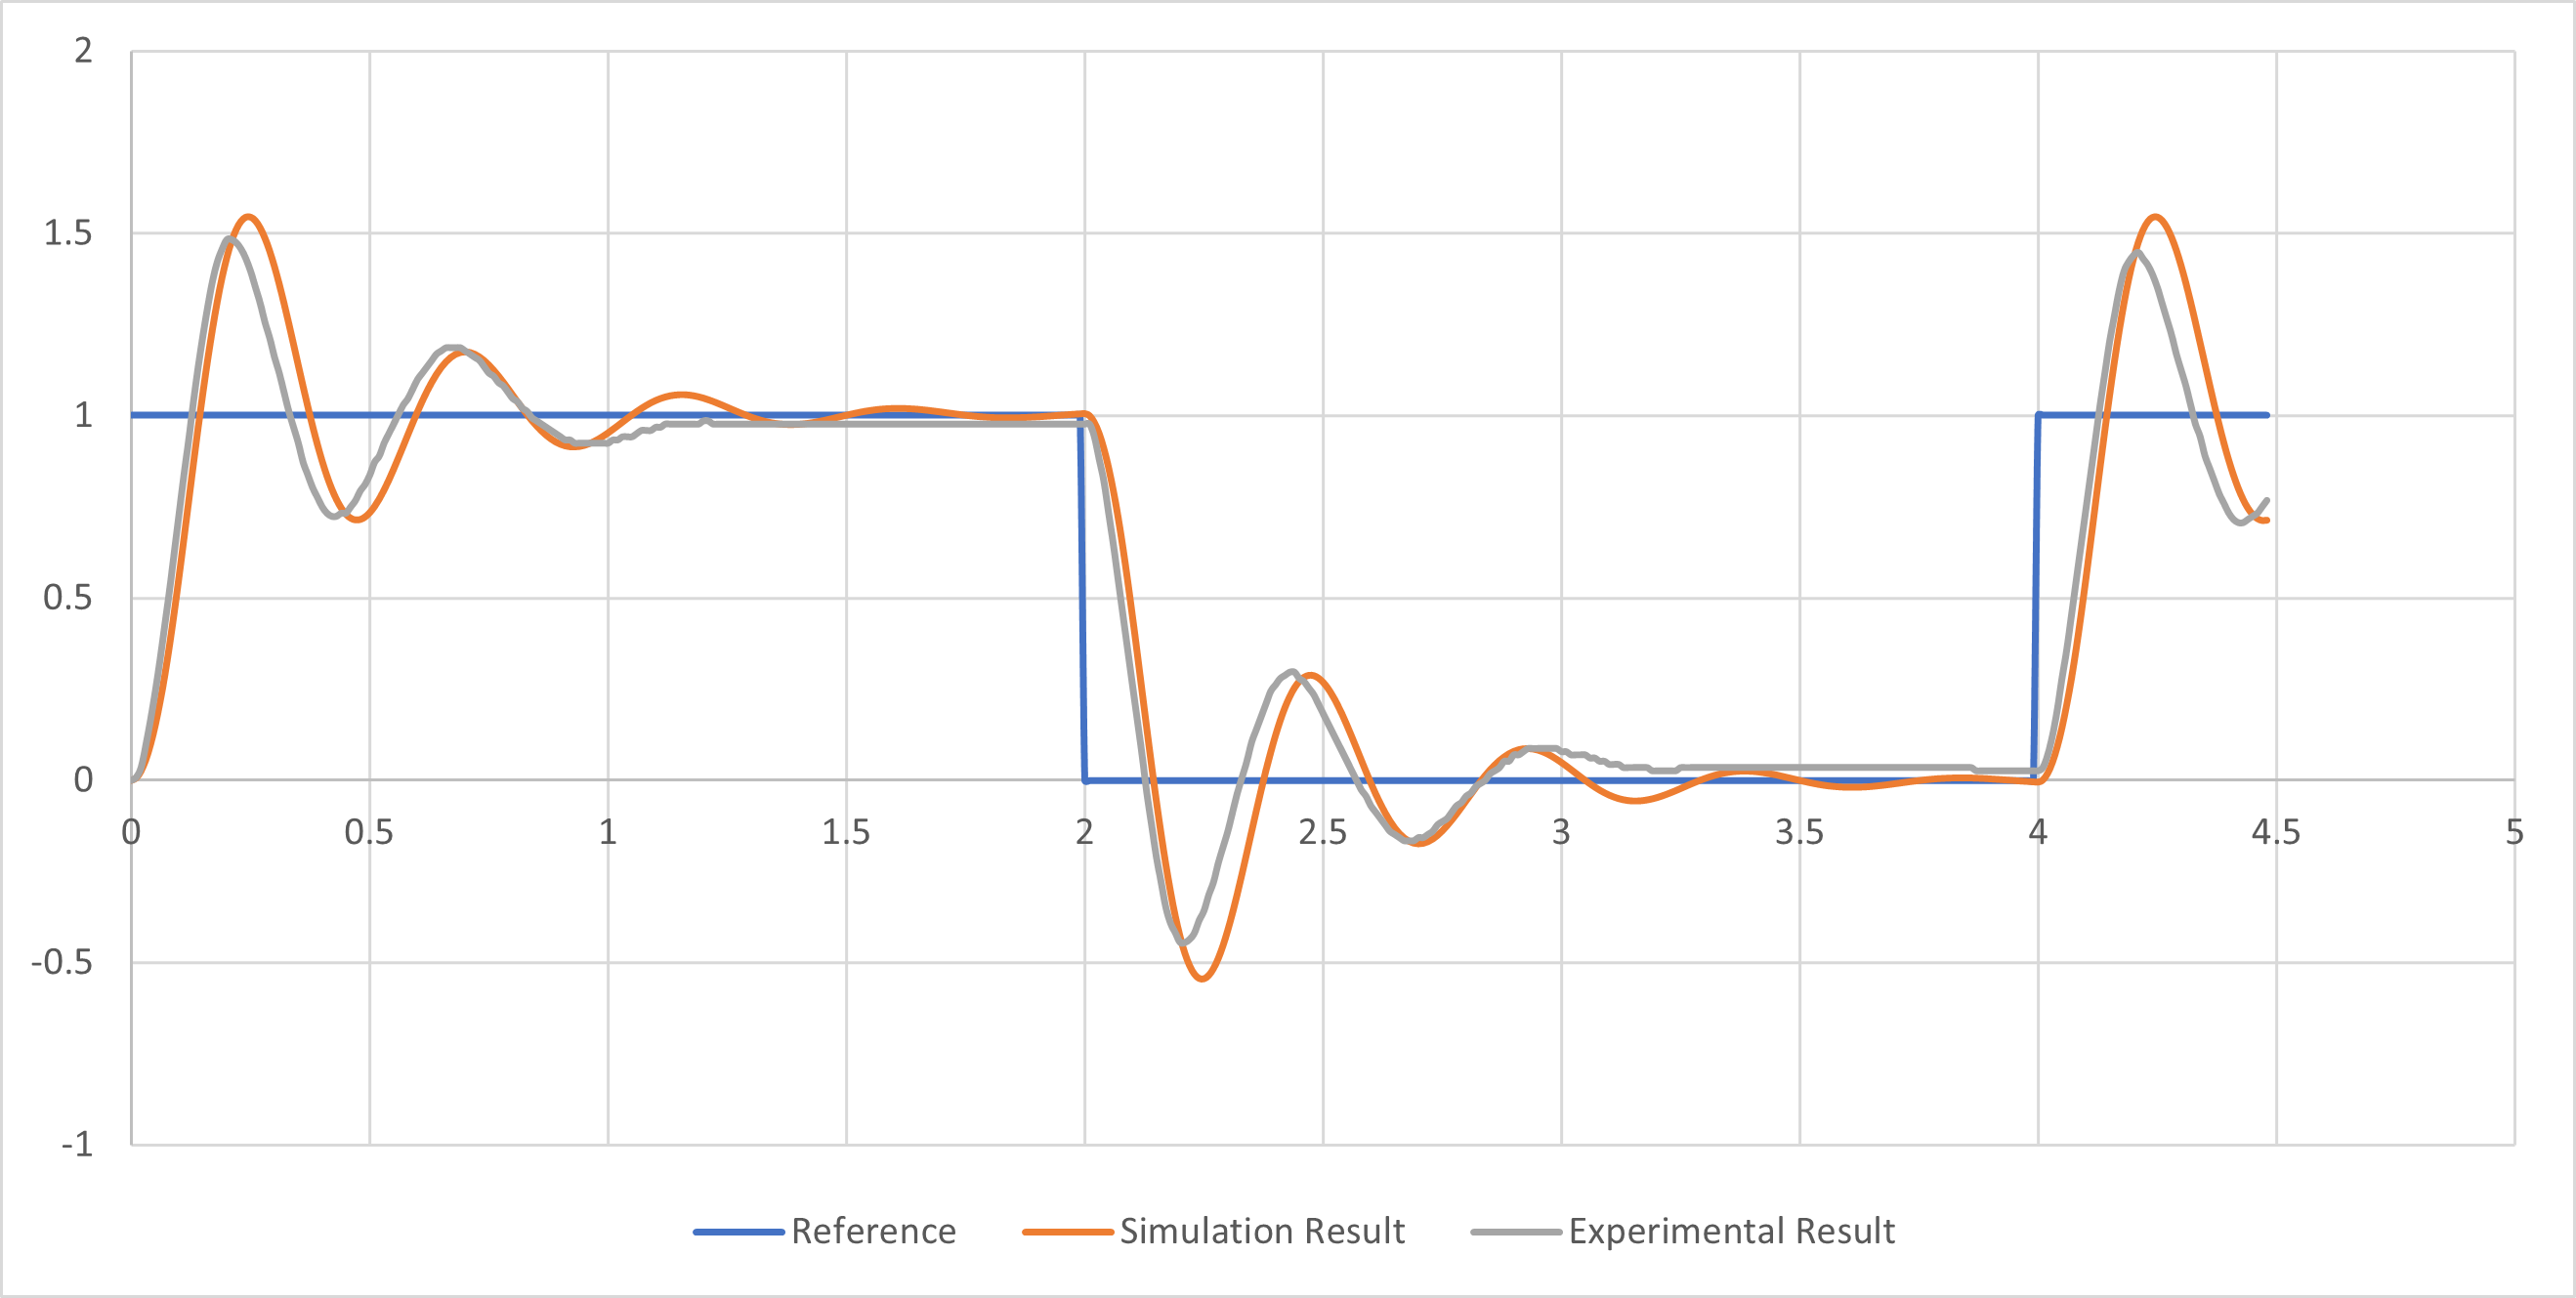
\includegraphics[scale=0.6]{023.png}
    \caption{$\alpha=1,K_{ff}=5.79$}
\end{figure}

\begin{figure}[h!]
    \centering
    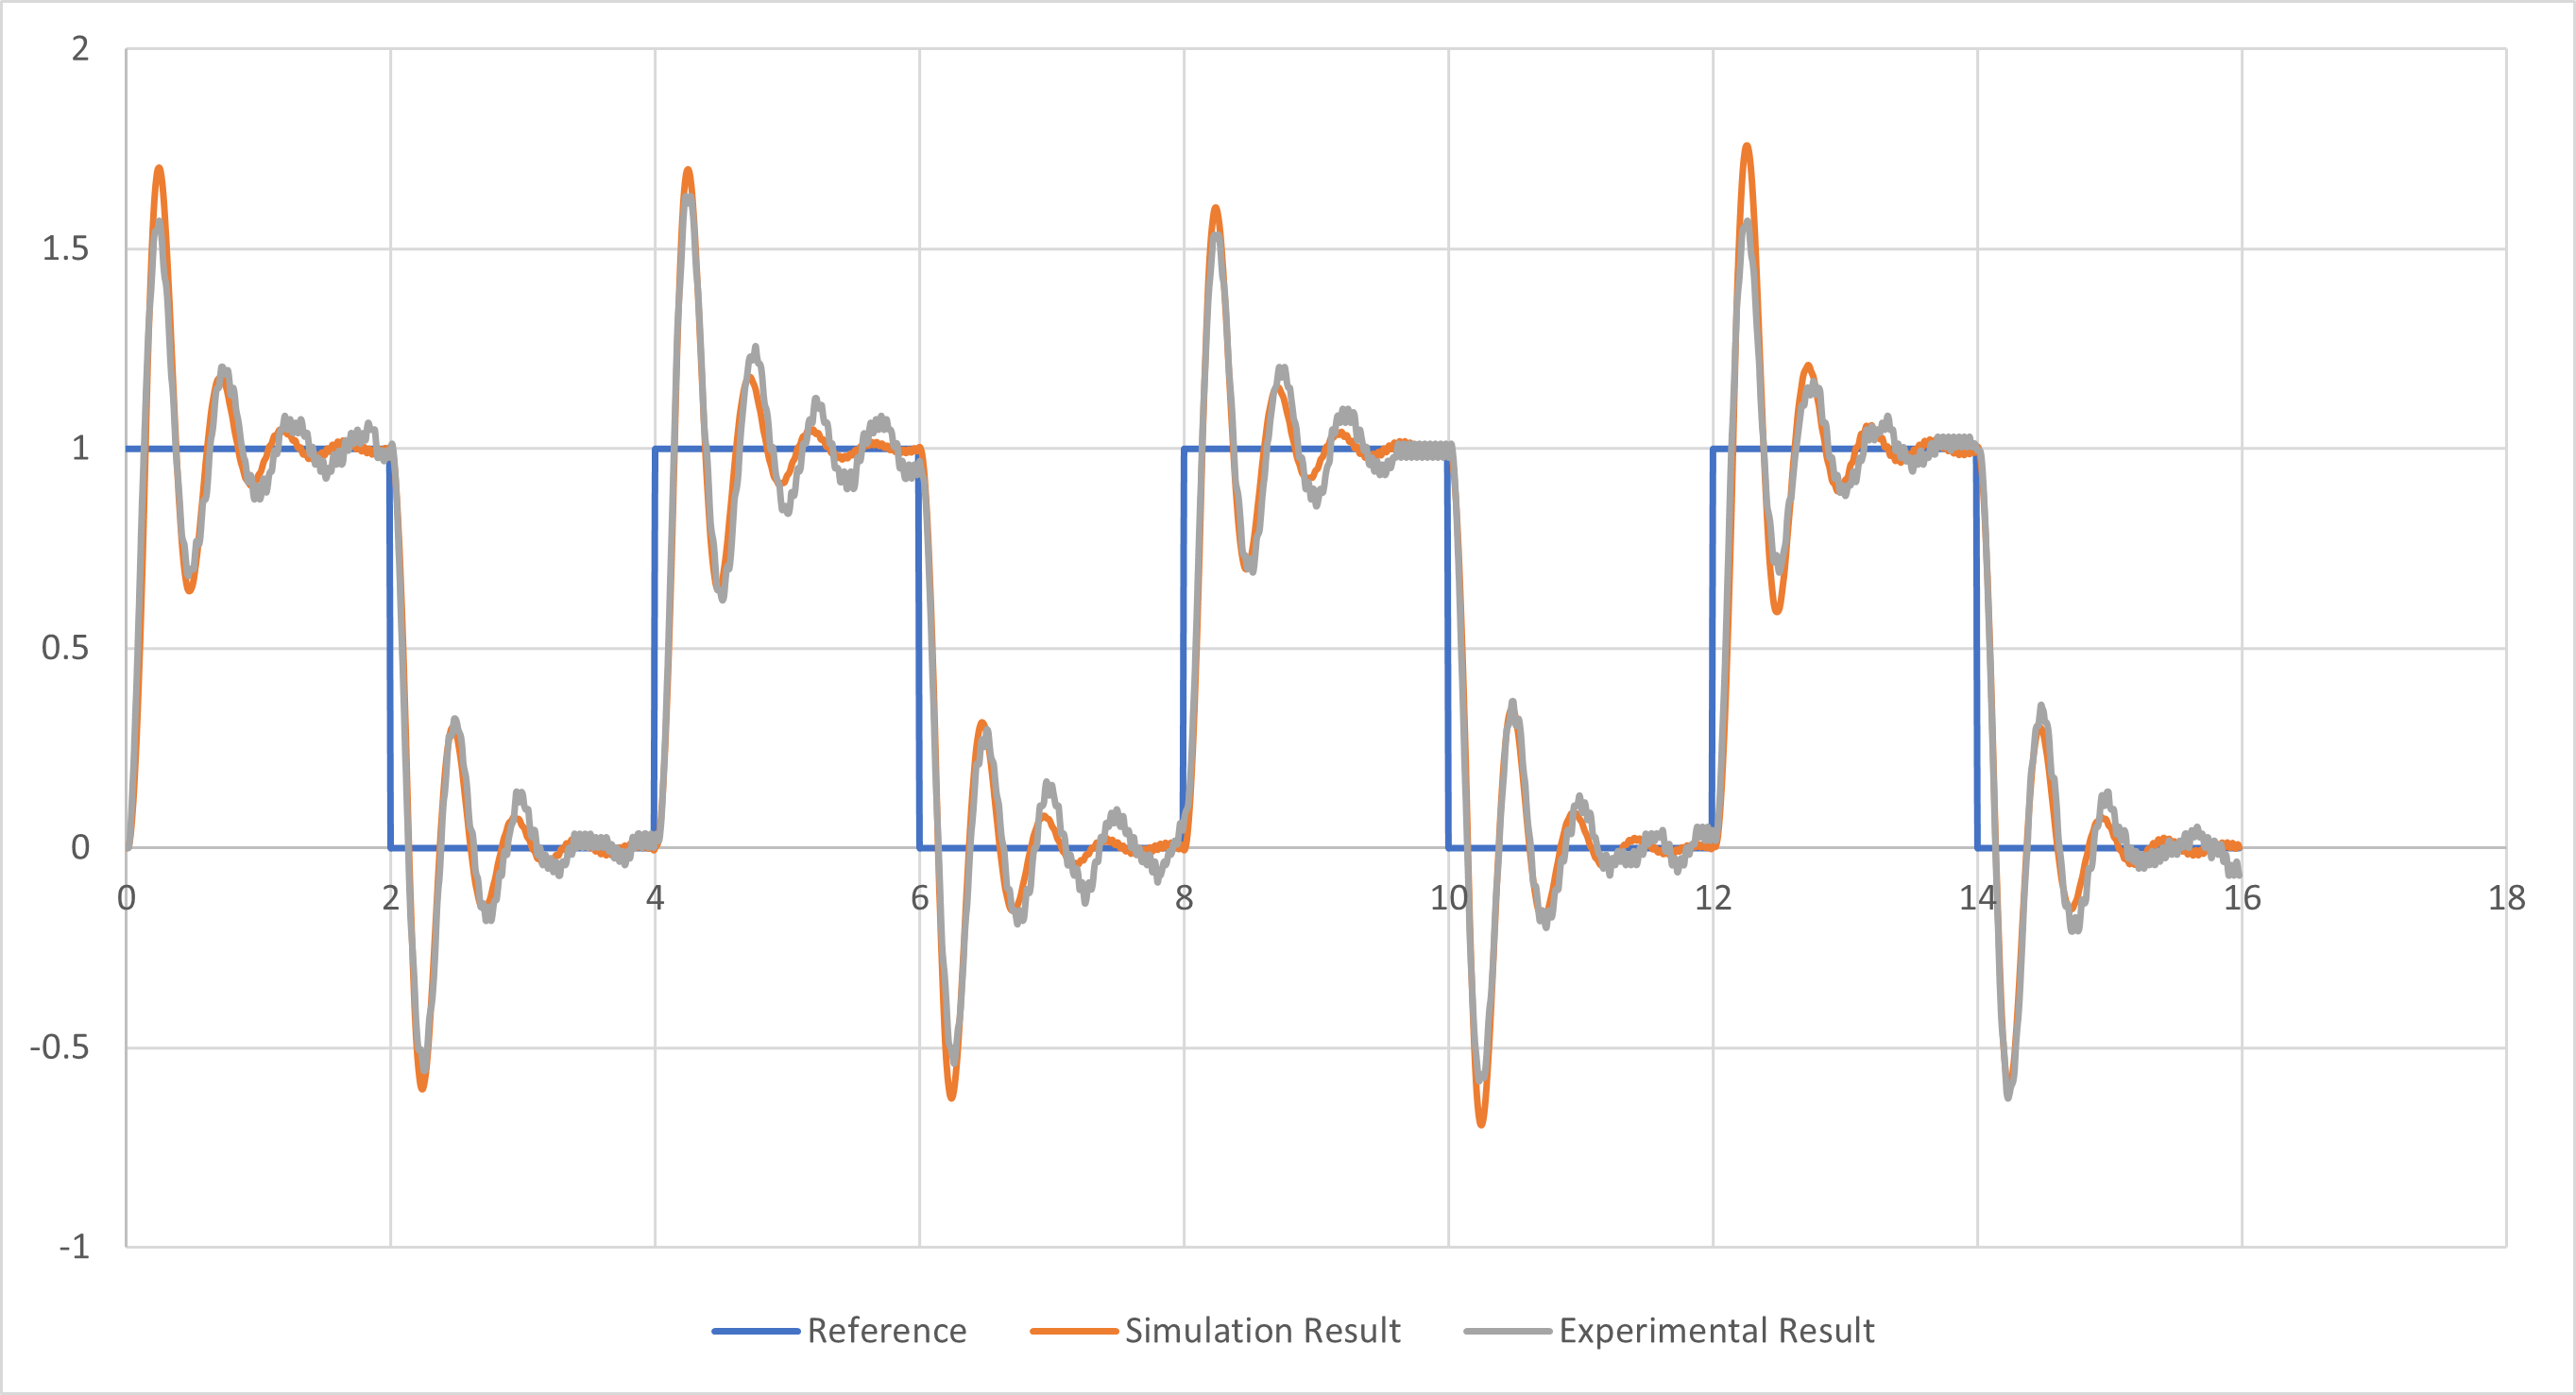
\includegraphics[scale=0.6]{024.png}
    \caption{$\alpha=200,K_{ff}=0$}
\end{figure}

\newpage

\subsection{制御性能評価}

得られた実験結果を最大絶対値誤差および二乗平均平方根誤差を計算する.

\begin{equation}
    e_{RMS}=\sqrt{\frac{1}{n}\sum_{i=1}^{n}e^{2}(i)},e(i)=\theta(i)-\hat{\theta}(i)
\end{equation}


\begin{table}[!htbp]
\centering
\caption{<最大絶対値誤差および二乗平均平方根誤差>}
\begin{tabular}{cccc}
\hline
 $ K_{ff}$ & $\alpha$ & $e_{RMS}$ & $e_{max}$\\
\hline
0& 20  & 0.028& 0.062\\
0& 1  & 0.051& 0.014\\
5.79 & 20 & 0.071& 0.218\\
5.79& 1 & 0.099&0.276\\
0 & 200 & 0.051 &0.189\\
\hline
\end{tabular}
\end{table}


最大絶対値誤差および二乗平均平方根誤差の計算によって、なるべく$\alpha$を大きく設定すると、プリレポートで計算したPIDパラメータの換算式によって、$K_{P},K_{I}$が大きくなり、$K_{D}$の値がわずか下って、制御性能も良くなっている.その一方で、$\alpha$も収束の速さが大きく影響している.$s=-\alpha$の極が収束の速度を支配しているから.フィードフォワード系を加えるとその影響がなくすことができる.しかし$\alpha$の絶対値を無限大に取ることができない.その理由はまず操作量の実験データから評価する.\\

フィードフォワード系を加えなく、$\alpha=1,20,200$の時の操作量をグラフにまとめる.



\begin{figure}[h!]
    \centering
    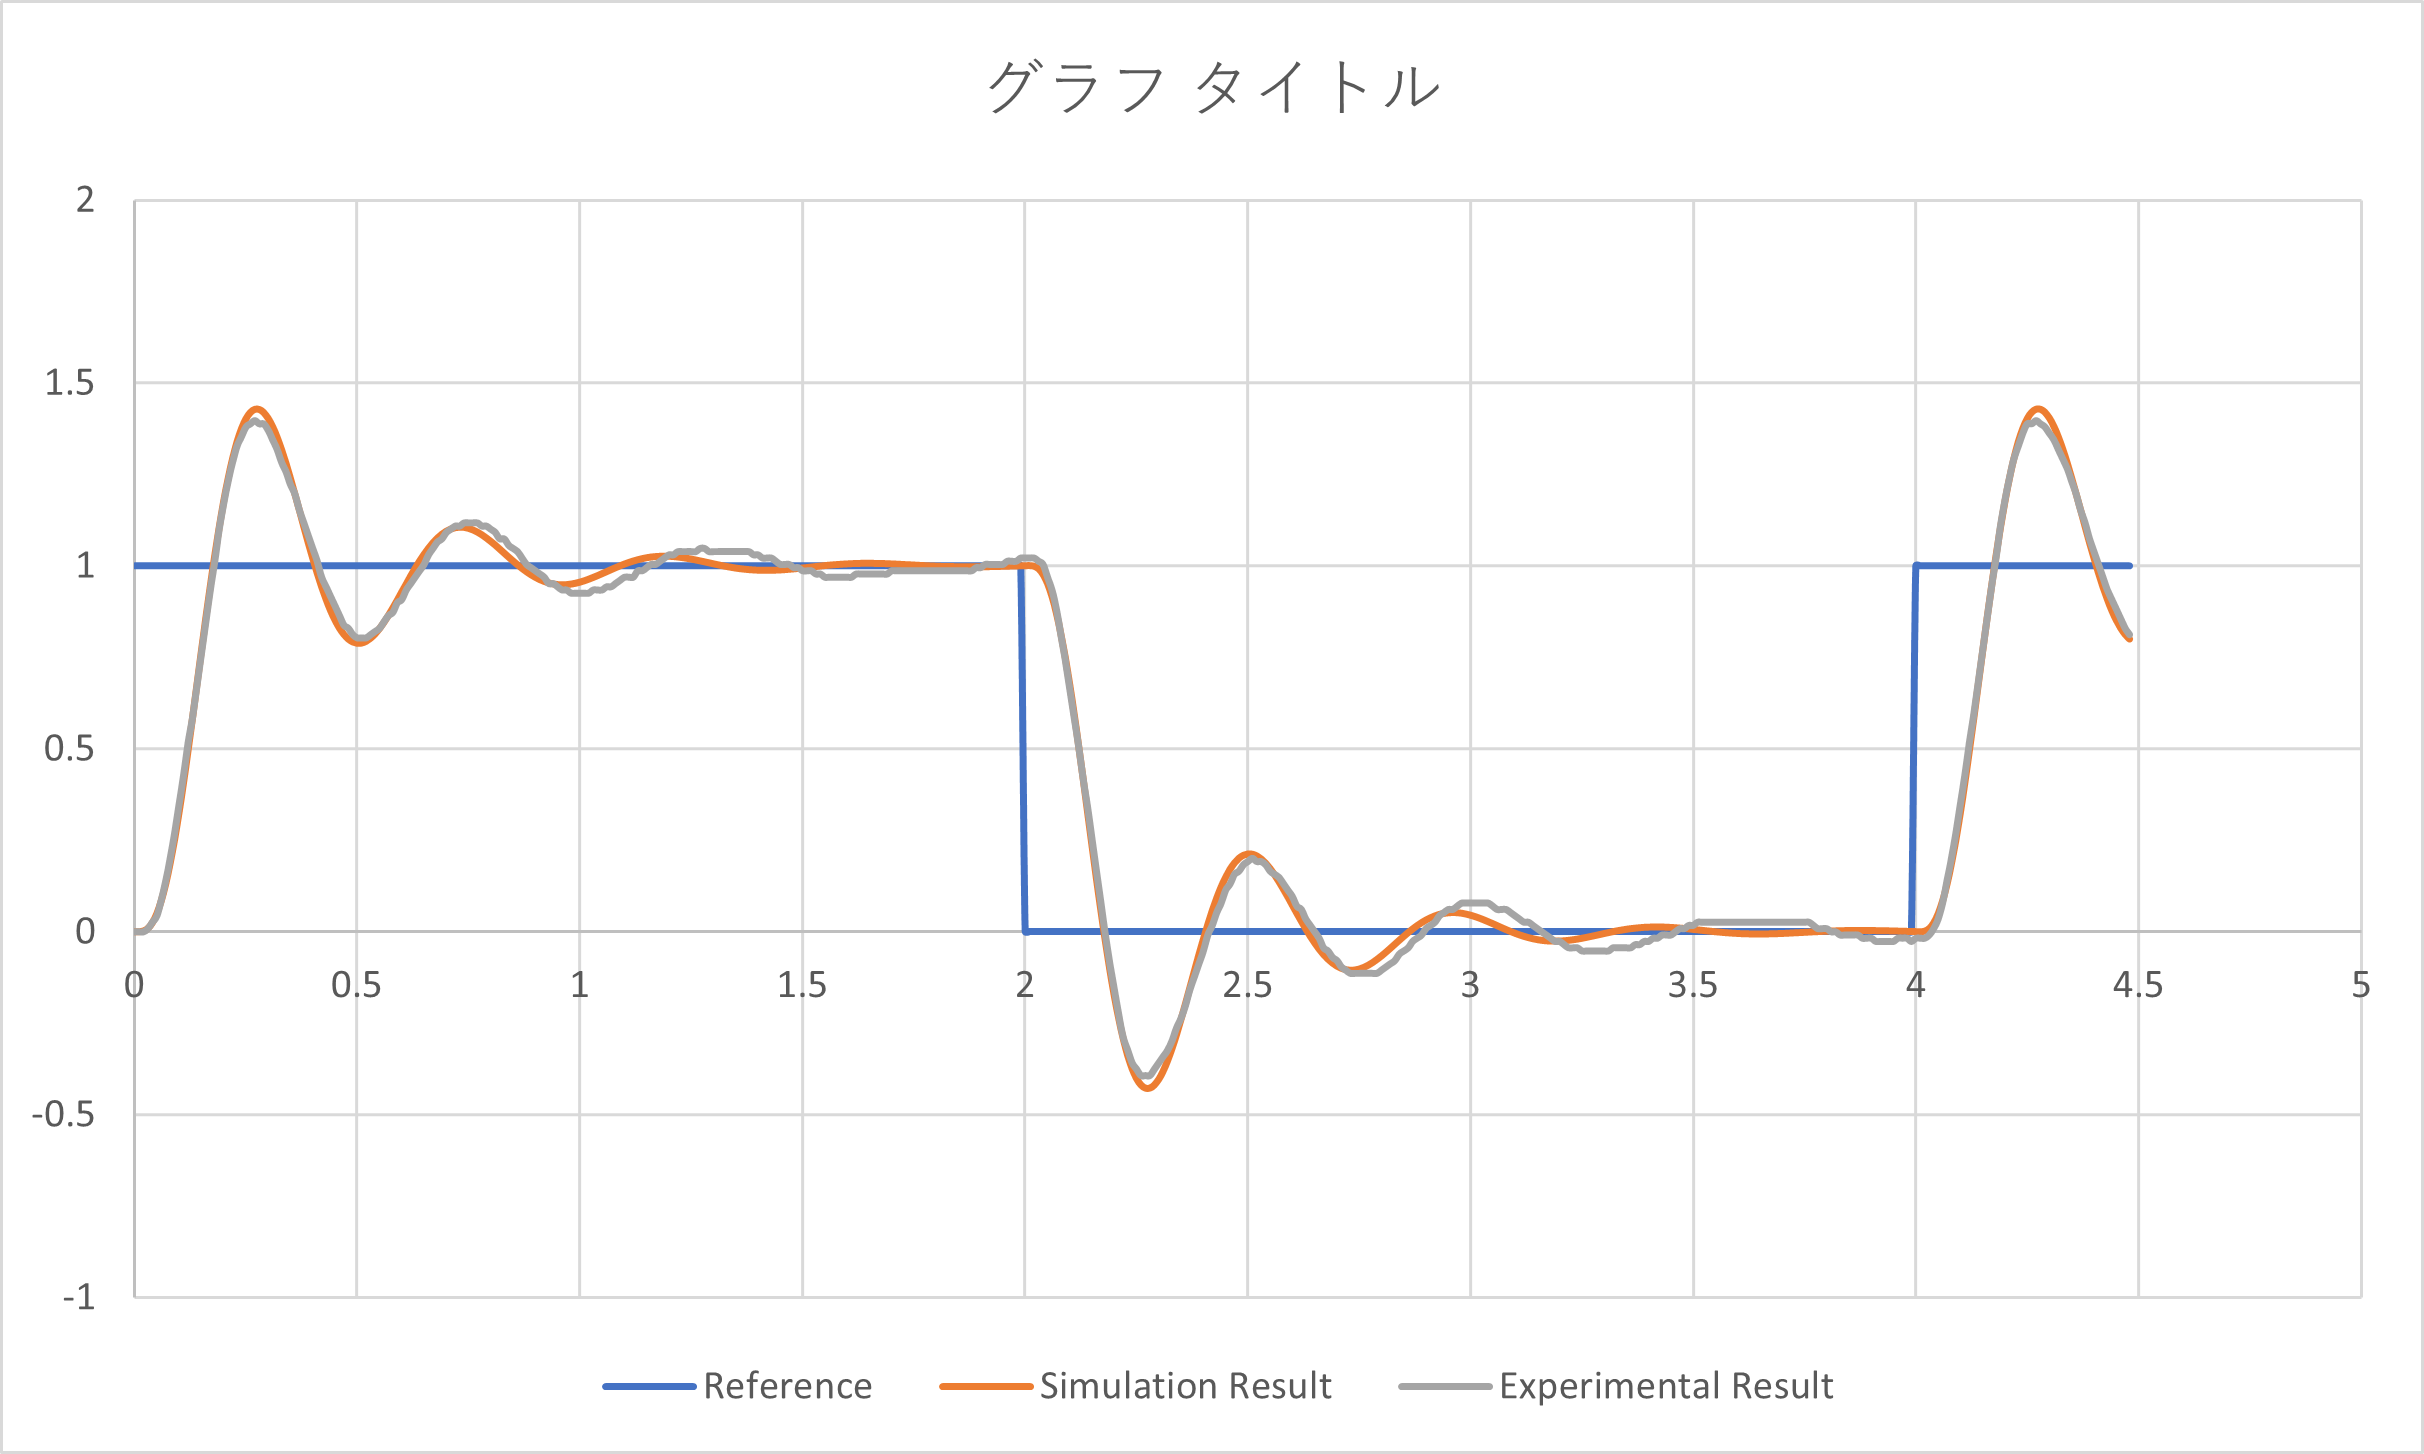
\includegraphics[scale=0.6]{020.png}
    \caption{$\alpha=20,K_{ff}=0$}
\end{figure}

\newpage

\begin{figure}[h!]
    \centering
    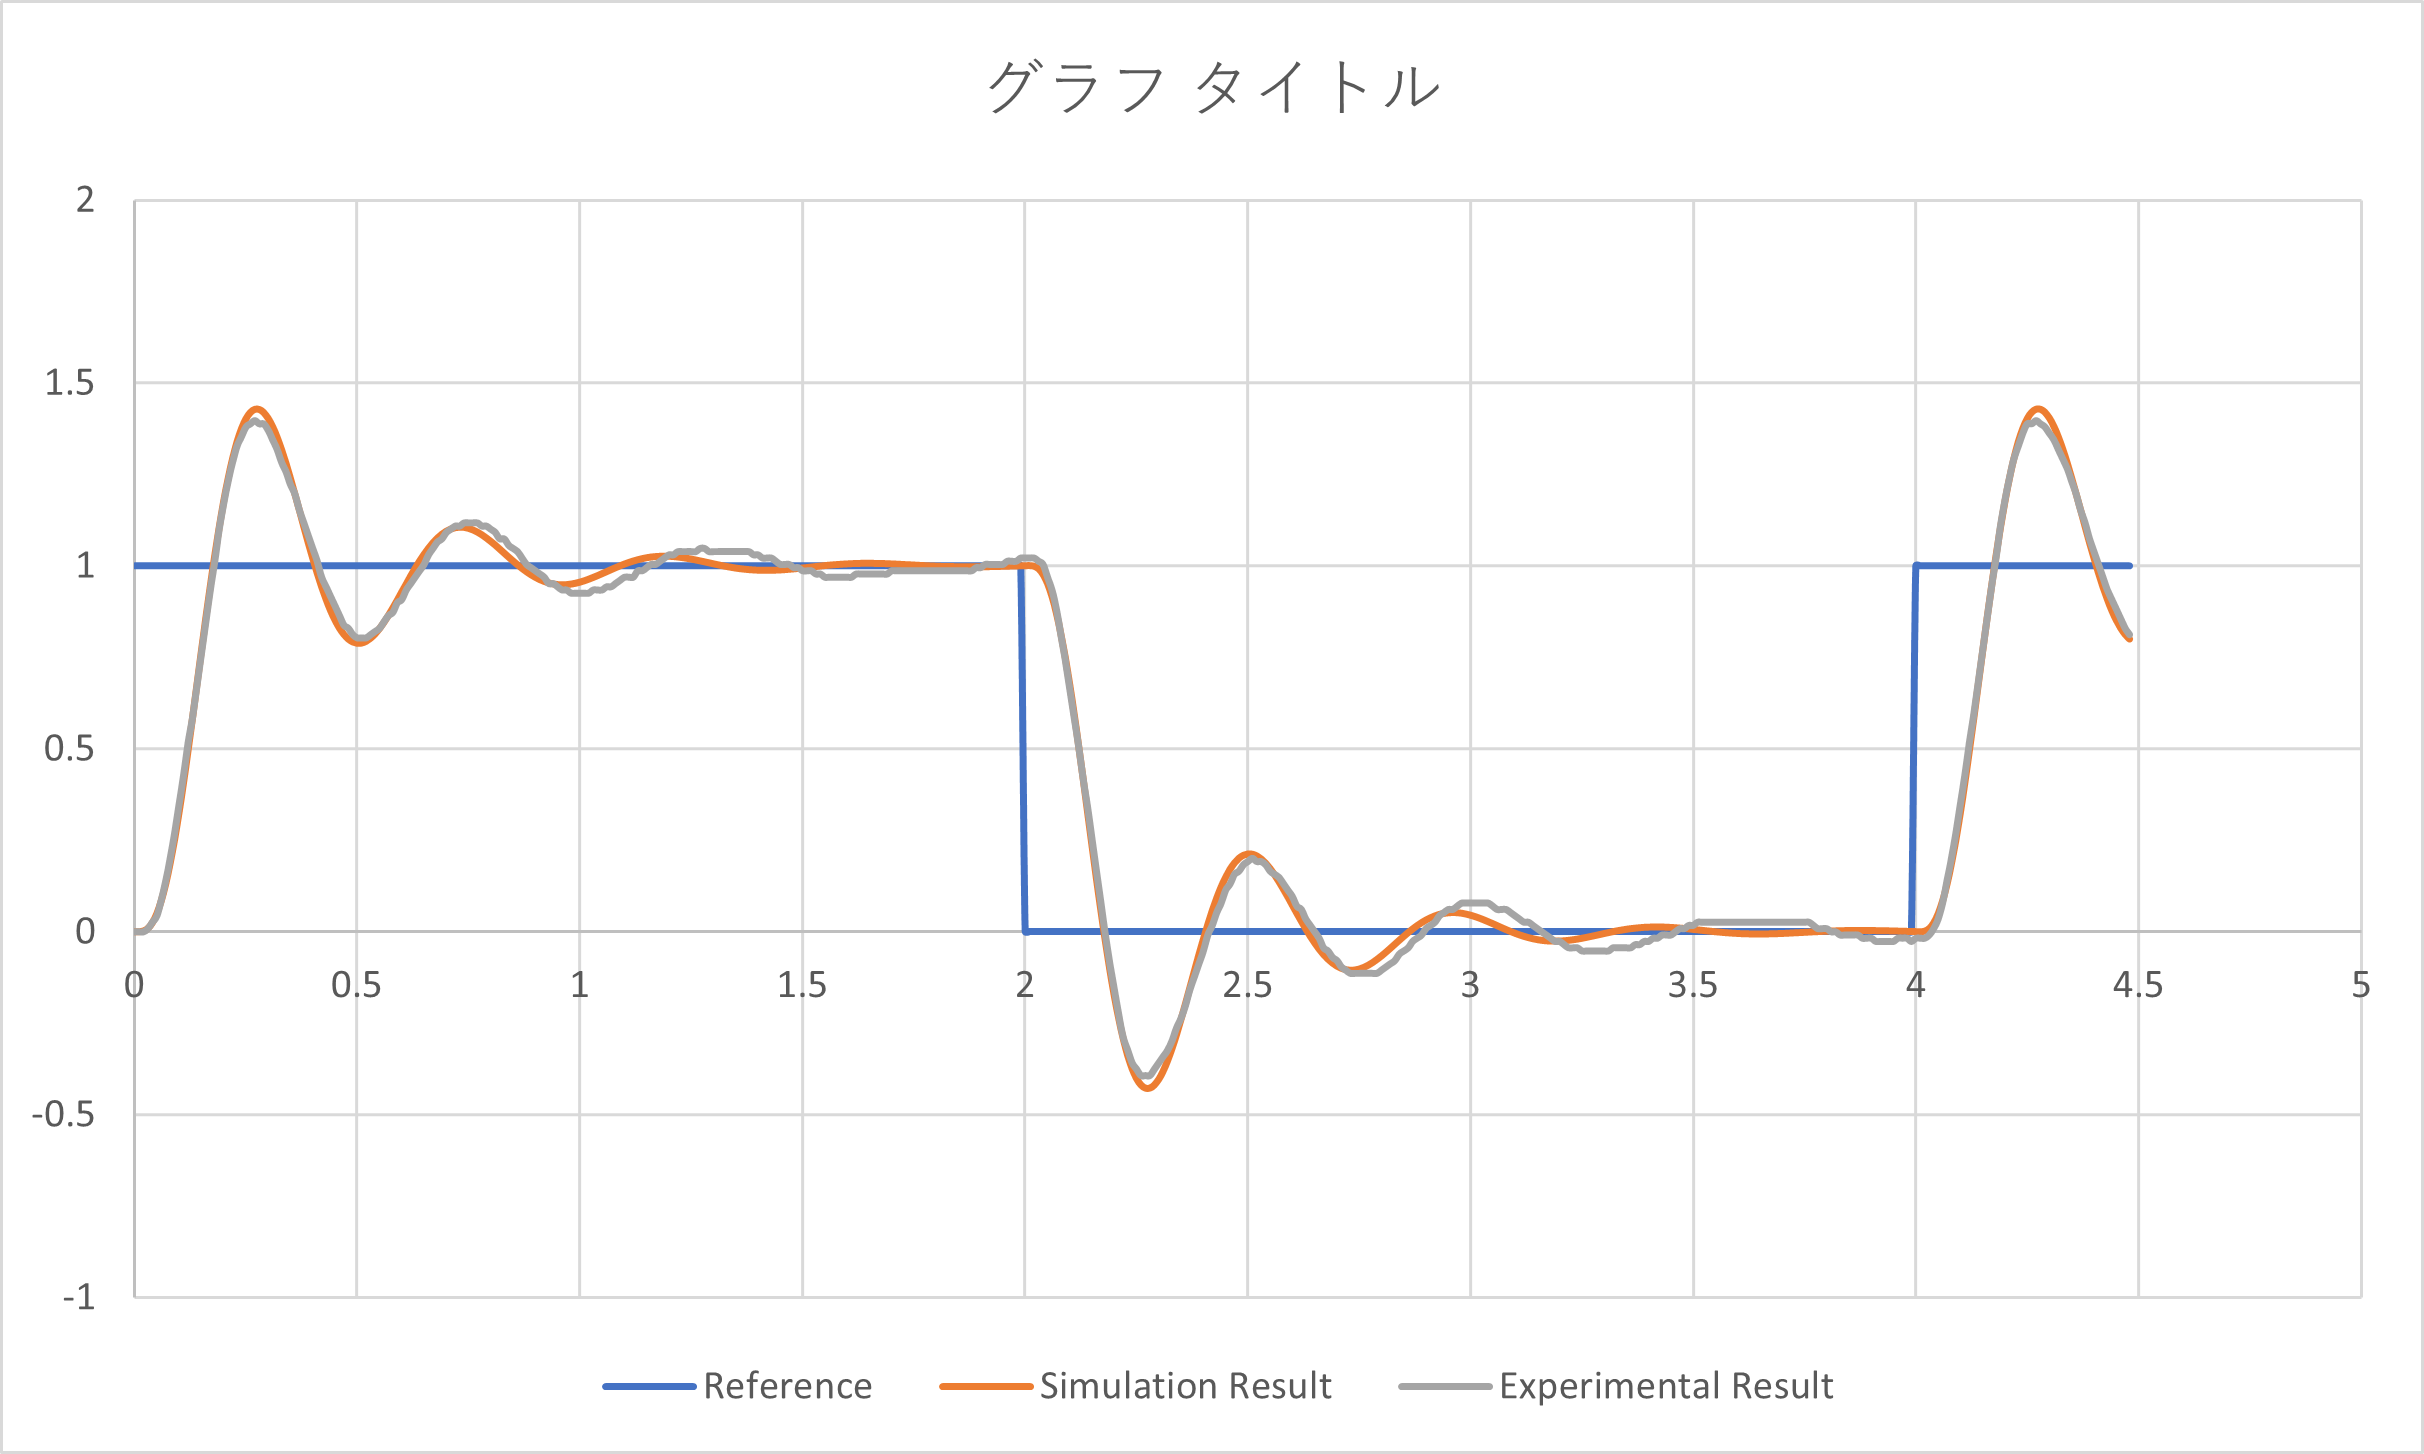
\includegraphics[scale=0.6]{020.png}
    \caption{$\alpha=20,K_{ff}=0$}
\end{figure}



\begin{figure}[h!]
    \centering
    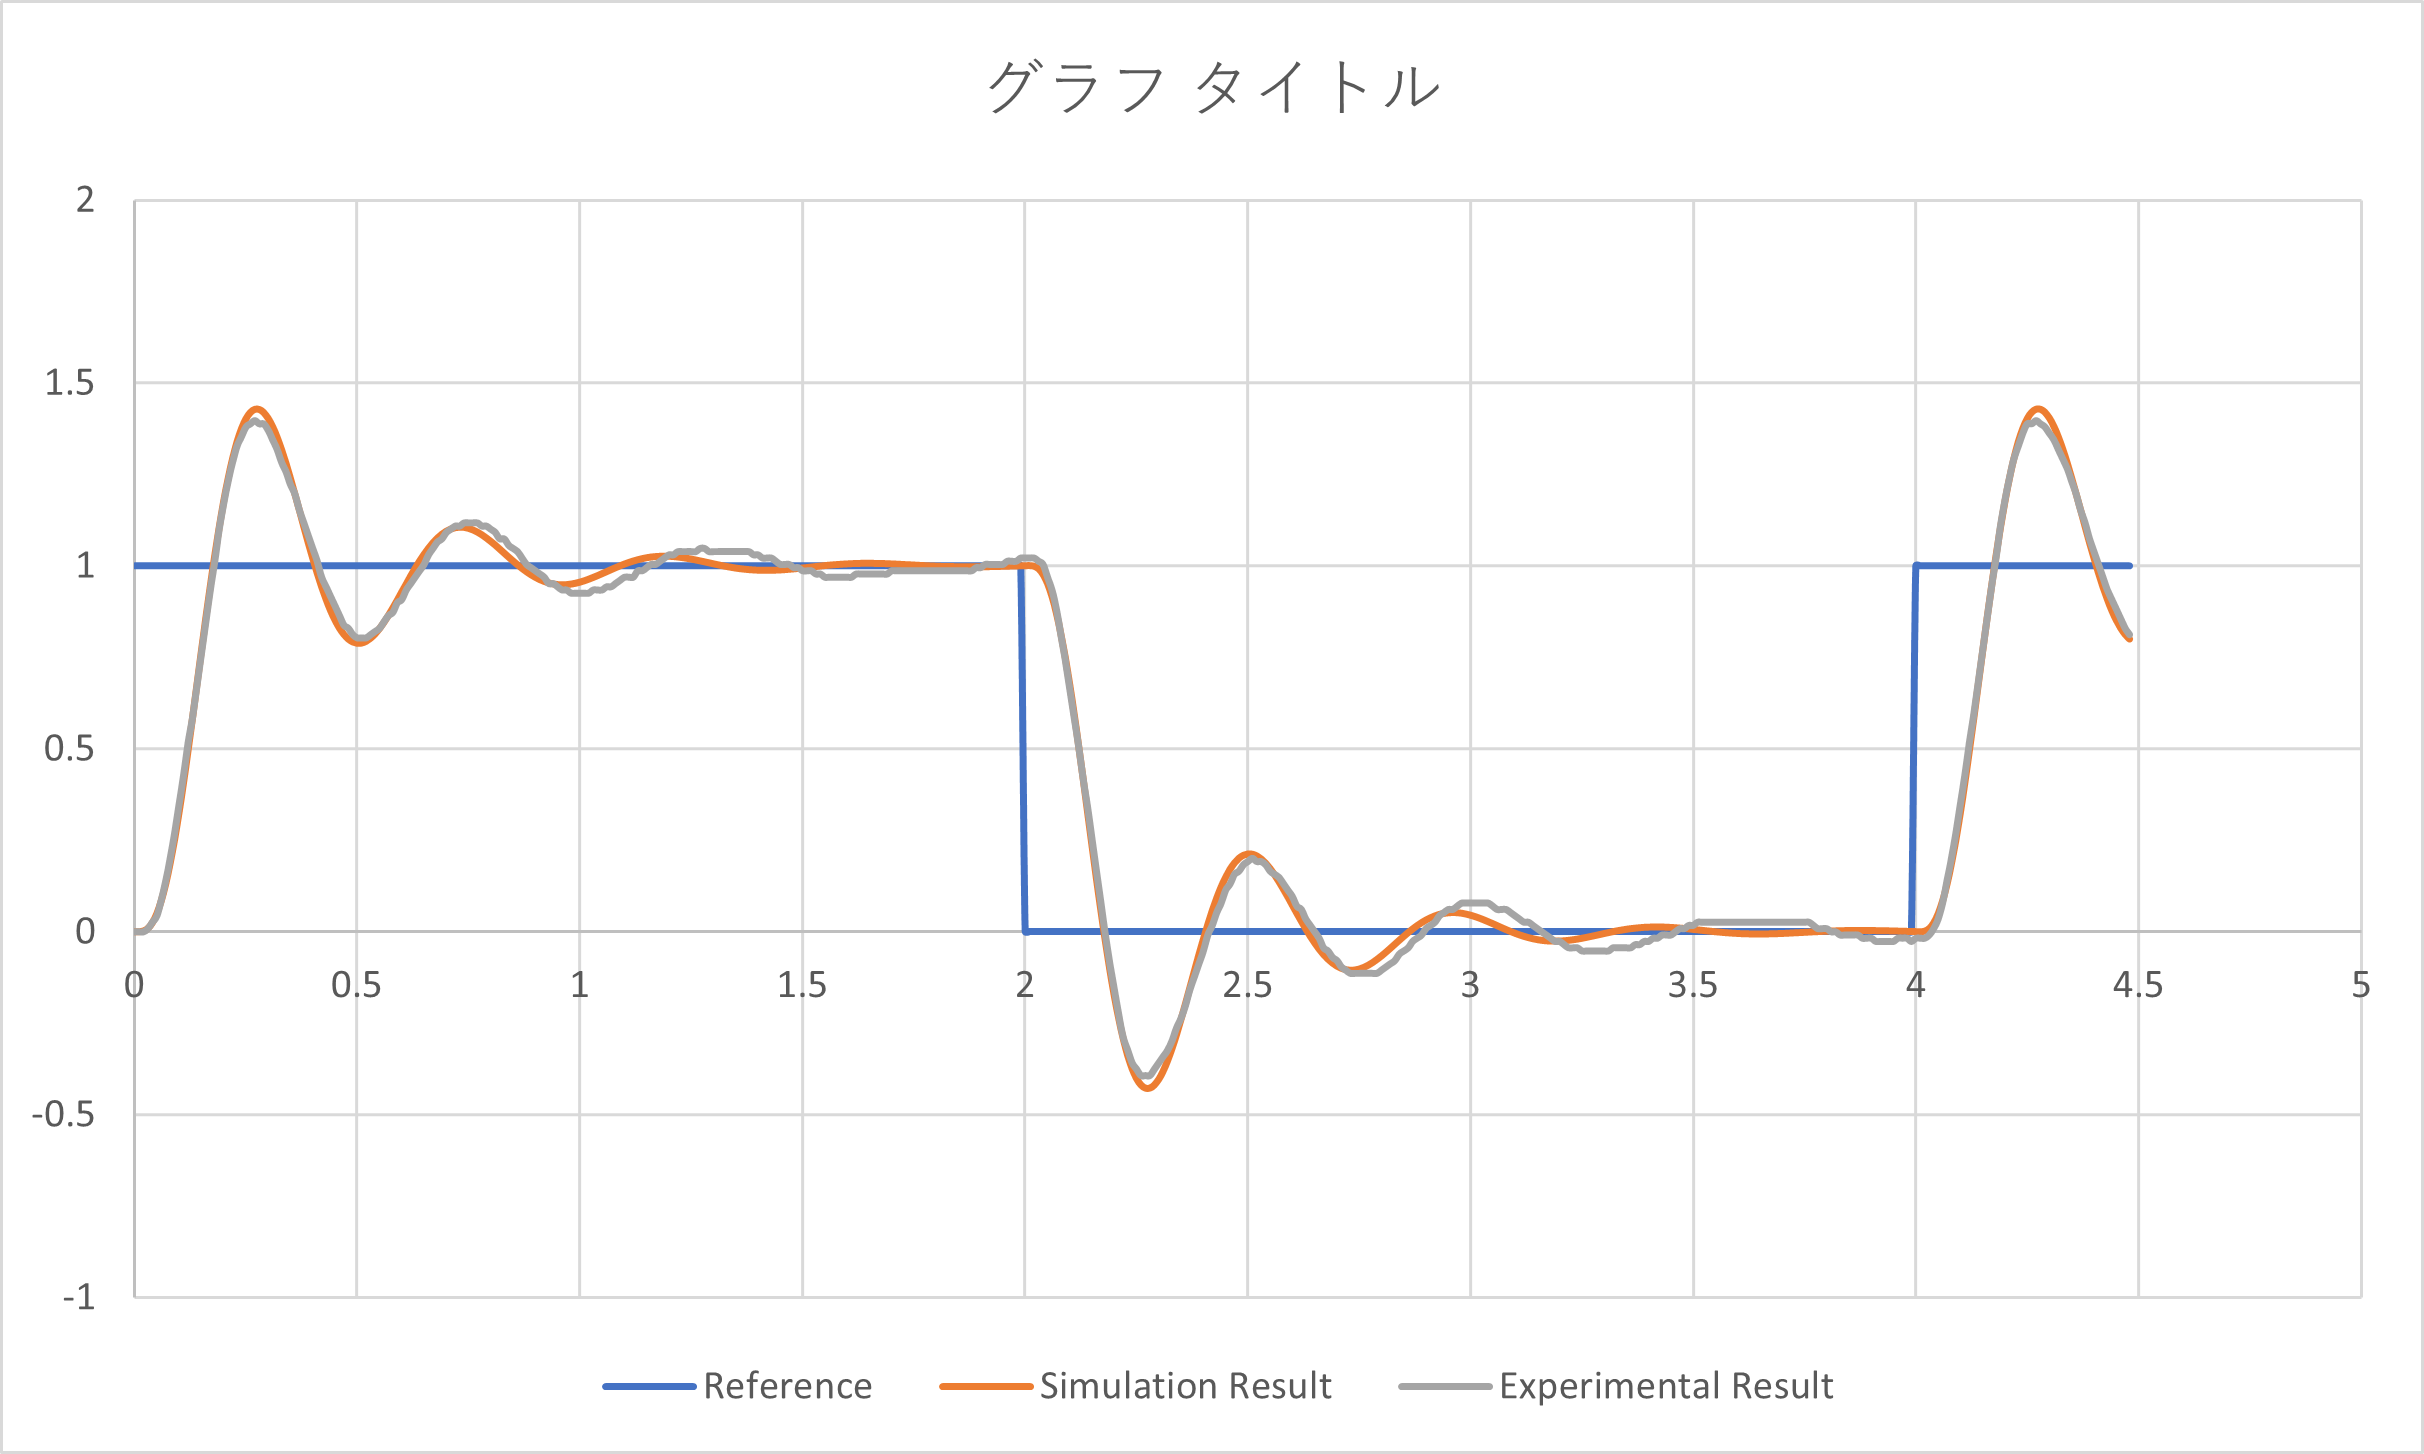
\includegraphics[scale=0.6]{020.png}
    \caption{$\alpha=20,K_{ff}=0$}
\end{figure}


    

\newpage


\section{課題}
(1)(i)モータ角度の制御性能評価は,最大絶対値誤差および二乗平均平方根誤差以外にはどのように
定量的に行うのが適切か.理由と合わせて述べよ.(ii) 3.4 節で得られた実験結果を上記に基づいて
評価せよ.\\



(2)フィードフォワード制御とフィードバック制御それぞれの効果および弱点の両方についてまとめよ.\\


(3)共振現象は機械システムおよび電気システムの両方で起きうるが,これらの工業的な応用例を各分野で 1 つずつ挙げ,図および式の両方を用いて原理を説明せよ.\\


(4)二次遅れ系の標準形において周波数応答におけるデシベルゲインが 1 より大きくなるのは,減衰係
数が $\sqrt{1/2}$よりも小さい場合であることを示せ.



\newpage

\begin{thebibliography}{9}
\bibitem{latexcompanion} 
日本機械学会,制御工学,JSMEテキストシリ,2010/8/31,p.19.20. 

\bibitem{latexcompanion} 
黒川一夫,ロボット用回路駆動設計,工学研究社,2007/10/22,p.4. 


\bibitem{einstein} 
Embedded Technology Lab,ワインドアップ現象とその対策,
\url{https://nagaoka-md.co.jp/2020/07/16/pmsm-foc-no9/},参考日:2020/11/4



\end{thebibliography}





\end{document}